\documentclass[11pt]{article}

\usepackage[margin=1in]{geometry}
\usepackage{graphicx}
\usepackage{booktabs}
\usepackage{amsmath}
\usepackage{tikz}
\usetikzlibrary{shapes.geometric, arrows.meta, positioning, calc}
\usepackage{enumitem}
\usepackage{pifont}
\usepackage{hyperref}

\title{\Large Appendix: HQF-DE Implementation Details}
\author{}
\date{}

\begin{document}

\maketitle

\appendix

\section{System Architecture}

Figure~\ref{fig:architecture} shows the overall HQF-DE system architecture with the four document variants flowing through both retrieval paths.

\begin{figure}[ht]
\centering
\resizebox{\textwidth}{!}{%
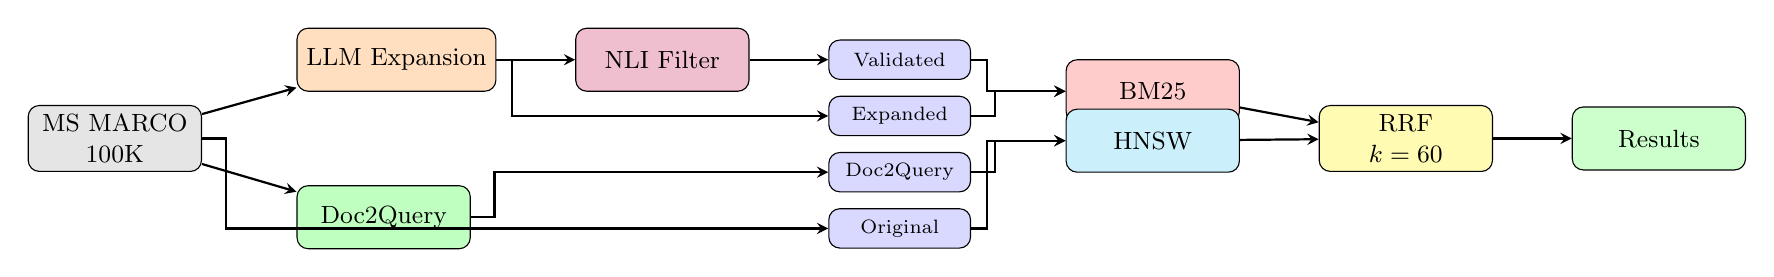
\begin{tikzpicture}[
    node distance=0.8cm,
    box/.style={rectangle, draw, rounded corners, minimum width=2.2cm, minimum height=0.8cm, align=center, font=\small},
    smallbox/.style={rectangle, draw, rounded corners, minimum width=1.8cm, minimum height=0.5cm, align=center, font=\scriptsize},
    arrow/.style={->, thick, >=stealth}
]
    % Input
    \node[box, fill=gray!20] (docs) {MS MARCO\\100K};

    % Expansion Methods
    \node[box, fill=orange!25, right=1.2cm of docs, yshift=1cm] (llm) {LLM Expansion};
    \node[box, fill=green!25, right=1.2cm of docs, yshift=-1cm] (d2q) {Doc2Query};

    % NLI
    \node[box, fill=purple!25, right=1cm of llm] (nli) {NLI Filter};

    % Variants
    \node[smallbox, fill=blue!15, right=1cm of nli] (v1) {Validated};
    \node[smallbox, fill=blue!15, below=0.2cm of v1] (v2) {Expanded};
    \node[smallbox, fill=blue!15, below=0.2cm of v2] (v3) {Doc2Query};
    \node[smallbox, fill=blue!15, below=0.2cm of v3] (v4) {Original};

    % Indexing
    \node[box, fill=red!20, right=1.2cm of v1, yshift=-0.4cm] (bm25) {BM25};
    \node[box, fill=cyan!20, right=1.2cm of v3, yshift=0.4cm] (hnsw) {HNSW};

    % Fusion
    \node[box, fill=yellow!30, right=1cm of bm25, yshift=-0.6cm] (rrf) {RRF\\$k=60$};

    % Output
    \node[box, fill=green!20, right=1cm of rrf] (out) {Results};

    % Arrows
    \draw[arrow] (docs) -- (llm);
    \draw[arrow] (docs) -- (d2q);
    \draw[arrow] (docs.east) -- ++(0.3,0) |- (v4.west);
    \draw[arrow] (llm) -- (nli);
    \draw[arrow] (llm.east) -- ++(0.2,0) |- (v2.west);
    \draw[arrow] (nli) -- (v1);
    \draw[arrow] (d2q.east) -- ++(0.3,0) |- (v3.west);

    \draw[arrow] (v1.east) -- ++(0.2,0) |- (bm25.west);
    \draw[arrow] (v2.east) -- ++(0.3,0) |- (bm25.west);
    \draw[arrow] (v3.east) -- ++(0.3,0) |- (hnsw.west);
    \draw[arrow] (v4.east) -- ++(0.2,0) |- (hnsw.west);

    \draw[arrow] (bm25) -- (rrf);
    \draw[arrow] (hnsw) -- (rrf);
    \draw[arrow] (rrf) -- (out);

\end{tikzpicture}
}
\caption{HQF-DE system architecture: document expansion variants flow through dual retrieval paths.}
\label{fig:architecture}
\end{figure}

\section{Pipeline Stages}

\begin{figure}[ht]
\centering
\resizebox{\textwidth}{!}{%
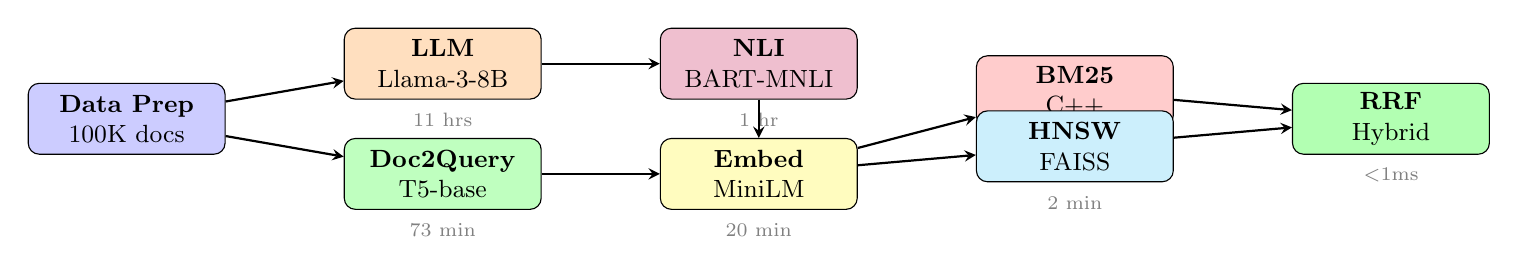
\begin{tikzpicture}[
    node distance=0.5cm and 1.2cm,
    stage/.style={rectangle, draw, rounded corners, minimum width=2.5cm, minimum height=0.9cm, align=center, font=\small},
    arrow/.style={->, thick, >=stealth},
    time/.style={font=\scriptsize, text=gray}
]
    % Row 1: Data + Expansion
    \node[stage, fill=blue!20] (data) {\textbf{Data Prep}\\100K docs};

    \node[stage, fill=orange!25, right=1.5cm of data, yshift=0.7cm] (llm) {\textbf{LLM}\\Llama-3-8B};
    \node[time, below=0.05cm of llm] {11 hrs};

    \node[stage, fill=green!25, right=1.5cm of data, yshift=-0.7cm] (d2q) {\textbf{Doc2Query}\\T5-base};
    \node[time, below=0.05cm of d2q] {73 min};

    % Row 2: NLI + Embeddings
    \node[stage, fill=purple!25, right=1.5cm of llm] (nli) {\textbf{NLI}\\BART-MNLI};
    \node[time, below=0.05cm of nli] {1 hr};

    \node[stage, fill=yellow!25, right=1.5cm of d2q] (embed) {\textbf{Embed}\\MiniLM};
    \node[time, below=0.05cm of embed] {20 min};

    % Row 3: Indexing
    \node[stage, fill=red!20, right=1.5cm of nli, yshift=-0.35cm] (bm25) {\textbf{BM25}\\C++};
    \node[time, below=0.05cm of bm25] {5 min};

    \node[stage, fill=cyan!20, right=1.5cm of embed, yshift=0.35cm] (hnsw) {\textbf{HNSW}\\FAISS};
    \node[time, below=0.05cm of hnsw] {2 min};

    % Row 4: Fusion
    \node[stage, fill=green!30, right=1.5cm of bm25, yshift=-0.35cm] (rrf) {\textbf{RRF}\\Hybrid};
    \node[time, below=0.05cm of rrf] {$<$1ms};

    % Arrows
    \draw[arrow] (data) -- (llm);
    \draw[arrow] (data) -- (d2q);
    \draw[arrow] (llm) -- (nli);
    \draw[arrow] (nli) -- (embed);
    \draw[arrow] (d2q) -- (embed);
    \draw[arrow] (embed) -- (bm25);
    \draw[arrow] (embed) -- (hnsw);
    \draw[arrow] (bm25) -- (rrf);
    \draw[arrow] (hnsw) -- (rrf);

\end{tikzpicture}
}
\caption{Pipeline stages with processing times. GPU stages run on Colab A100; CPU stages run locally.}
\label{fig:pipeline}
\end{figure}

\section{Infrastructure Adaptation}

Due to GPU memory constraints on local hardware, we adopted a hybrid execution approach.

\begin{figure}[ht]
\centering
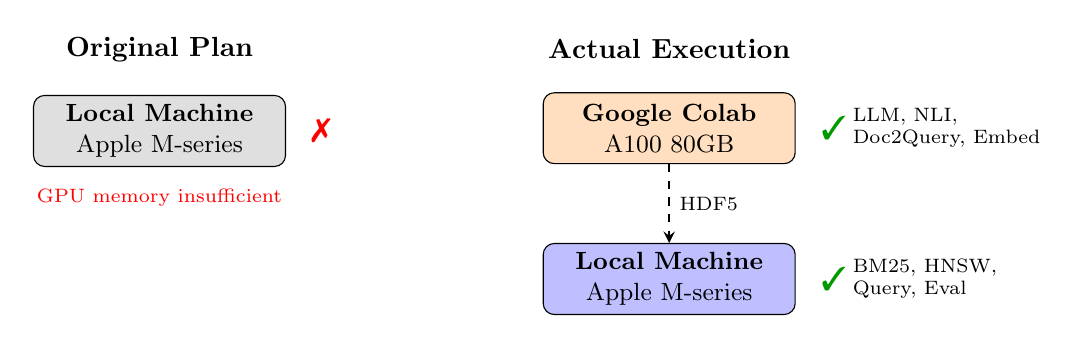
\begin{tikzpicture}[
    node distance=0.6cm,
    box/.style={rectangle, draw, rounded corners, minimum width=3.2cm, minimum height=0.9cm, align=center, font=\small},
    arrow/.style={->, thick, >=stealth, dashed},
    check/.style={font=\large, text=green!60!black},
    cross/.style={font=\large, text=red}
]
    % Original Plan
    \node[font=\bfseries] (t1) {Original Plan};
    \node[box, fill=gray!25, below=0.3cm of t1] (local1) {\textbf{Local Machine}\\Apple M-series};
    \node[cross, right=0.2cm of local1] {\ding{55}};
    \node[font=\scriptsize, text=red, below=0.15cm of local1] {GPU memory insufficient};

    % Actual
    \node[font=\bfseries, right=3.5cm of t1] (t2) {Actual Execution};
    \node[box, fill=orange!25, below=0.3cm of t2] (colab) {\textbf{Google Colab}\\A100 80GB};
    \node[check, right=0.2cm of colab] {\ding{51}};

    \node[box, fill=blue!25, below=1cm of colab] (local2) {\textbf{Local Machine}\\Apple M-series};
    \node[check, right=0.2cm of local2] {\ding{51}};

    % Tasks
    \node[font=\scriptsize, right=0.6cm of colab, text width=2.5cm, align=left] {
        LLM, NLI,\\Doc2Query, Embed
    };

    \node[font=\scriptsize, right=0.6cm of local2, text width=2.5cm, align=left] {
        BM25, HNSW,\\Query, Eval
    };

    % Data transfer
    \draw[arrow] (colab) -- node[right, font=\scriptsize] {HDF5} (local2);

\end{tikzpicture}
\caption{Infrastructure adaptation: GPU tasks on Colab, CPU tasks locally.}
\label{fig:infra}
\end{figure}

\section{Complexity Summary}

\begin{table}[ht]
\centering
\caption{Time and Space Complexity of Key Components}
\begin{tabular}{lcc}
\toprule
\textbf{Component} & \textbf{Time} & \textbf{Space} \\
\midrule
BM25 Indexing & $O(N \cdot L)$ & $O(V + P)$ \\
BM25 Query & $O(\sum_{t} |L_t|)$ & $O(k)$ \\
HNSW Construction & $O(N \log N \cdot M)$ & $O(N \cdot M \cdot \log N)$ \\
HNSW Query & $O(\log N + k \cdot ef)$ & $O(ef)$ \\
RRF Fusion & $O(k_1 + k_2)$ & $O(k_1 + k_2)$ \\
\bottomrule
\end{tabular}
\label{tab:complexity}

\vspace{0.2cm}
\footnotesize
\textit{$N$=docs, $L$=doc length, $V$=vocab, $P$=postings, $|L_t|$=posting list, $M$=connections, $ef$=beam width}
\end{table}

\section{Complete Results}

\subsection{HNSW Dense Retrieval}

\begin{table}[ht]
\centering
\caption{HNSW Results (MRR@10 / nDCG@10 / Recall@100)}
\begin{tabular}{lccc}
\toprule
\textbf{Variant} & \textbf{TREC 2019} & \textbf{TREC 2020} & \textbf{Dev Set} \\
\midrule
Original & 0.374 / 0.154 / 0.485 & 0.275 / 0.105 / 0.551 & 0.011 / 0.002 / 0.876 \\
Expanded & \textbf{0.447} / \textbf{0.154} / 0.471 & 0.273 / 0.094 / 0.550 & 0.012 / 0.003 / 0.866 \\
Validated & 0.381 / 0.149 / 0.472 & 0.267 / 0.092 / 0.551 & 0.013 / 0.004 / 0.869 \\
Doc2Query & 0.305 / 0.134 / 0.472 & \textbf{0.307} / 0.085 / 0.540 & 0.013 / 0.003 / 0.865 \\
\bottomrule
\end{tabular}
\end{table}

\subsection{BM25 Sparse Retrieval}

\begin{table}[ht]
\centering
\caption{BM25 Results (MRR@10 / nDCG@10 / Recall@100)}
\begin{tabular}{lccc}
\toprule
\textbf{Variant} & \textbf{TREC 2019} & \textbf{TREC 2020} & \textbf{Dev Set} \\
\midrule
Original & 0.744 / 0.419 / 0.568 & 0.688 / 0.428 / 0.590 & 0.689 / 0.712 / 0.933 \\
Expanded & 0.752 / 0.428 / 0.579 & 0.713 / 0.412 / 0.602 & 0.658 / 0.685 / 0.908 \\
Validated & 0.736 / 0.415 / 0.578 & 0.703 / 0.411 / 0.601 & 0.662 / 0.689 / 0.911 \\
Doc2Query & \textbf{0.844} / \textbf{0.492} / \textbf{0.596} & \textbf{0.741} / \textbf{0.465} / \textbf{0.628} & \textbf{0.746} / \textbf{0.767} / \textbf{0.944} \\
\bottomrule
\end{tabular}
\end{table}

\subsection{Hybrid Retrieval (RRF)}

\begin{table}[ht]
\centering
\caption{Hybrid Results (MRR@10 / nDCG@10 / Recall@100)}
\begin{tabular}{lccc}
\toprule
\textbf{Variant} & \textbf{TREC 2019} & \textbf{TREC 2020} & \textbf{Dev Set} \\
\midrule
Original & 0.877 / 0.475 / 0.594 & 0.757 / 0.431 / 0.641 & 0.701 / 0.730 / 0.945 \\
Expanded & 0.810 / 0.459 / 0.588 & 0.723 / 0.412 / 0.636 & 0.676 / 0.707 / 0.923 \\
Validated & 0.810 / 0.451 / 0.587 & 0.719 / 0.410 / 0.635 & 0.680 / 0.709 / 0.926 \\
Doc2Query & \textbf{0.896} / \textbf{0.512} / \textbf{0.613} & \textbf{0.779} / \textbf{0.468} / \textbf{0.653} & \textbf{0.762} / \textbf{0.783} / \textbf{0.951} \\
\bottomrule
\end{tabular}
\end{table}

\section{Key Findings Visualization}

\begin{figure}[ht]
\centering
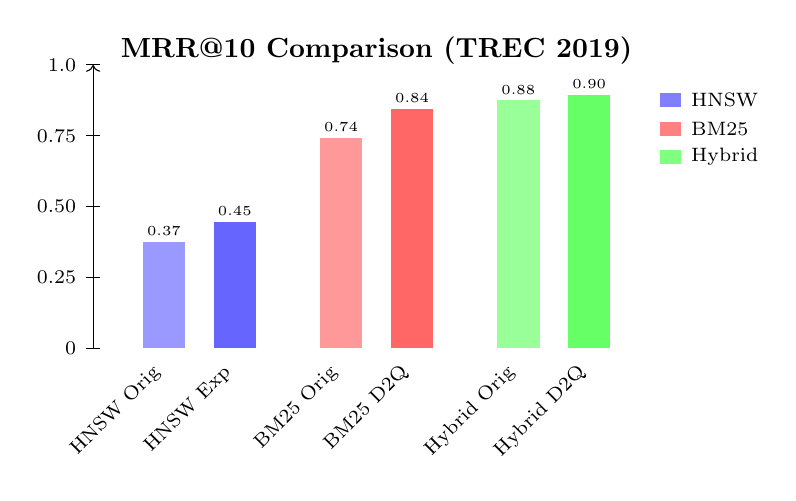
\begin{tikzpicture}[scale=0.9]
    % Title
    \node[font=\bfseries] at (4, 4.2) {MRR@10 Comparison (TREC 2019)};

    % Y-axis
    \draw[->] (0,0) -- (0,4);
    \foreach \y/\val in {0/0, 1/0.25, 2/0.50, 3/0.75, 4/1.0} {
        \draw (-0.1,\y) -- (0.1,\y);
        \node[left, font=\scriptsize] at (-0.1,\y) {\val};
    }

    % Bars - HNSW
    \node[font=\scriptsize, rotate=45, anchor=east] at (1,-0.2) {HNSW Orig};
    \fill[blue!40] (0.7,0) rectangle (1.3,1.50);
    \node[font=\tiny] at (1,1.65) {0.37};

    \node[font=\scriptsize, rotate=45, anchor=east] at (2,-0.2) {HNSW Exp};
    \fill[blue!60] (1.7,0) rectangle (2.3,1.79);
    \node[font=\tiny] at (2,1.94) {0.45};

    % Bars - BM25
    \node[font=\scriptsize, rotate=45, anchor=east] at (3.5,-0.2) {BM25 Orig};
    \fill[red!40] (3.2,0) rectangle (3.8,2.97);
    \node[font=\tiny] at (3.5,3.12) {0.74};

    \node[font=\scriptsize, rotate=45, anchor=east] at (4.5,-0.2) {BM25 D2Q};
    \fill[red!60] (4.2,0) rectangle (4.8,3.38);
    \node[font=\tiny] at (4.5,3.53) {0.84};

    % Bars - Hybrid
    \node[font=\scriptsize, rotate=45, anchor=east] at (6,-0.2) {Hybrid Orig};
    \fill[green!40] (5.7,0) rectangle (6.3,3.50);
    \node[font=\tiny] at (6,3.65) {0.88};

    \node[font=\scriptsize, rotate=45, anchor=east] at (7,-0.2) {Hybrid D2Q};
    \fill[green!60] (6.7,0) rectangle (7.3,3.58);
    \node[font=\tiny] at (7,3.73) {0.90};

    % Legend
    \fill[blue!50] (8,3.4) rectangle (8.3,3.6);
    \node[right, font=\scriptsize] at (8.3,3.5) {HNSW};
    \fill[red!50] (8,3.0) rectangle (8.3,3.2);
    \node[right, font=\scriptsize] at (8.3,3.1) {BM25};
    \fill[green!50] (8,2.6) rectangle (8.3,2.8);
    \node[right, font=\scriptsize] at (8.3,2.7) {Hybrid};

\end{tikzpicture}
\caption{MRR@10 comparison. Hybrid + Doc2Query achieves best performance (0.90).}
\label{fig:mrr_comparison}
\end{figure}

\section{Expansion Method Comparison}

\begin{figure}[ht]
\centering
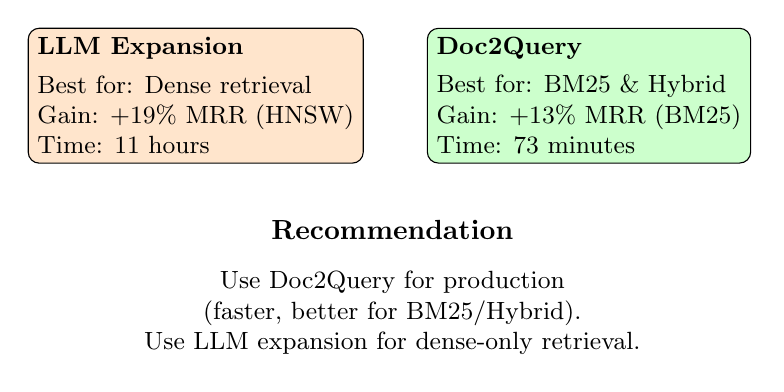
\begin{tikzpicture}[
    box/.style={rectangle, draw, rounded corners, minimum width=3.8cm, minimum height=1.6cm, align=left, font=\small}
]
    \node[box, fill=orange!20] (llm) {
        \textbf{LLM Expansion}\\[0.1cm]
        Best for: Dense retrieval\\
        Gain: +19\% MRR (HNSW)\\
        Time: 11 hours
    };

    \node[box, fill=green!20, right=0.8cm of llm] (d2q) {
        \textbf{Doc2Query}\\[0.1cm]
        Best for: BM25 \& Hybrid\\
        Gain: +13\% MRR (BM25)\\
        Time: 73 minutes
    };

    \node[font=\bfseries, below=0.6cm of $(llm.south)!0.5!(d2q.south)$] (rec) {Recommendation};
    \node[font=\small, below=0.15cm of rec, text width=9cm, align=center] {
        Use Doc2Query for production (faster, better for BM25/Hybrid).\\
        Use LLM expansion for dense-only retrieval.
    };

\end{tikzpicture}
\caption{Expansion method comparison with practical recommendations.}
\label{fig:expansion_comparison}
\end{figure}

\section{AI Assistance}

Claude and Gemini were used to assist with code development, debugging, and \LaTeX{} formatting throughout this project.

\end{document}
